% =====================================================================
% Appendix
% =====================================================================

\section{Notation}
\label{app:notation}

\begin{table}[h]
\centering
\caption{Notation used throughout the paper.}
\label{tab:notation}
\small
\setlength{\tabcolsep}{6pt}
\begin{tabular}{@{}ll@{}}
\toprule
Symbol & Meaning \\
\midrule
$x,\ y_b,\ s_{b,t}$ & Prompt; response $y_b=(y_{b,1},\dots,y_{b,T_b})$; state $s_{b,t}=(x,y_{b,1},\dots,y_{b,t-1})$. \\
$b,\ t,\ j$ & Response index; token index; absolute trainer-update index. \\
$T_b,\ \mathcal T_{\mathrm{act}}$ & Length of response $b$; active (non-padding) token positions of the microbatch. \\
$\mu_{b,t}$ & Behavior policy, namely the distribution the rollout engine actually sampled token $(b,t)$ from. \\
$\pi^{(j)}$ & Current trainer policy at update $j$. \\
$\pi^{(\ell)}$ & Trainer-side reference log-probability at the rollout checkpoint. \\
$n,\ N_{b,t}$ & Configured pipeline lag (trainer steps per weight broadcast); realized per-token lag. \\
$r_{b,t},\ d_{b,t}$ & Sampled-token importance ratio and its log-ratio, $d_{b,t}=\log r_{b,t}$. \\
$\rho^{\mathrm{seq}}_b$ & GSPO length-normalized sequence ratio in Equation~\eqref{eq:gspo-ratio}. \\
$\hat A_{b,t},\ R(y),\ \xi$ & Advantage estimate; sequence reward; reward bound with $|R(y)|\le\xi$. \\
$\dtv$ & Per-state total variation $\tfrac12\sum_a|\mu(a\mid s)-\pi(a\mid s)|$. \\
$L'_{\mu}(\pi)$ & Finite-horizon linear surrogate in Equation~\eqref{eq:surrogate}. \\
$\elow,\ \ehigh$ & Base clip radii; $\tilde\varepsilon_{\mathrm{low}/\mathrm{high},b,t}$ are the \satr{} radii in Equation~\eqref{eq:adaptive-eps}. \\
$\psi(u;q),\ q,\ c_{\pm,b,t}$ & Hill kernel; detached microbatch quantile reference; gated contraction factors. \\
$\dpi$ & Sampled training--inference mismatch $\E_{(b,t)\in\mathcal T_{\mathrm{act}}}|\log r^{\mathrm{tok}}_{b,t}|$ from Equation~\eqref{eq:mismatch-metric}. \\
\bottomrule
\end{tabular}
\end{table}

\section{Synchronization Regimes of Asynchronous RL}
\label{app:regimes}

The main text now keeps only the batch-wise asynchronous pipeline in Figure~\ref{fig:pipeline}, because all reported experiments are conducted in that regime. This appendix records the two endpoint cases referenced there---Appendix~\ref{app:sync-rl} for synchronous RL and Appendix~\ref{app:fully-async} for fully asynchronous RL. They clarify why the configured lag is only a coarse systems label and why the realized mismatch can vary substantially even when the nominal training recipe stays fixed.

\subsection{Synchronous RL}
\label{app:sync-rl}

In synchronous RL, rollout and optimization alternate on one shared GPU pool and every batch is trained by the same parameter vector that produced it:
\begin{equation}
j=\ell,
\qquad
\theta_{\mathrm{roll}}=\theta_{\mathrm{train}}=\theta^{(\ell)},
\qquad
N_{b,t}=0,
\qquad
\mu_{b,t}=\pi^{(\ell)},
\qquad
r_{b,t}=1\ \text{a.s.}
\label{eq:sync-identity}
\end{equation}
At this pre-update behavior point, the sampled ratio carries no off-policy correction, and under the usual on-policy assumptions the surrogate gradient coincides with the corresponding policy-gradient estimator. This regime therefore removes staleness as a learning issue, but it pays a clear systems cost: generation, optimization, and weight broadcast are serialized, so the two engines never overlap.

\begin{figure}[h]
\centering
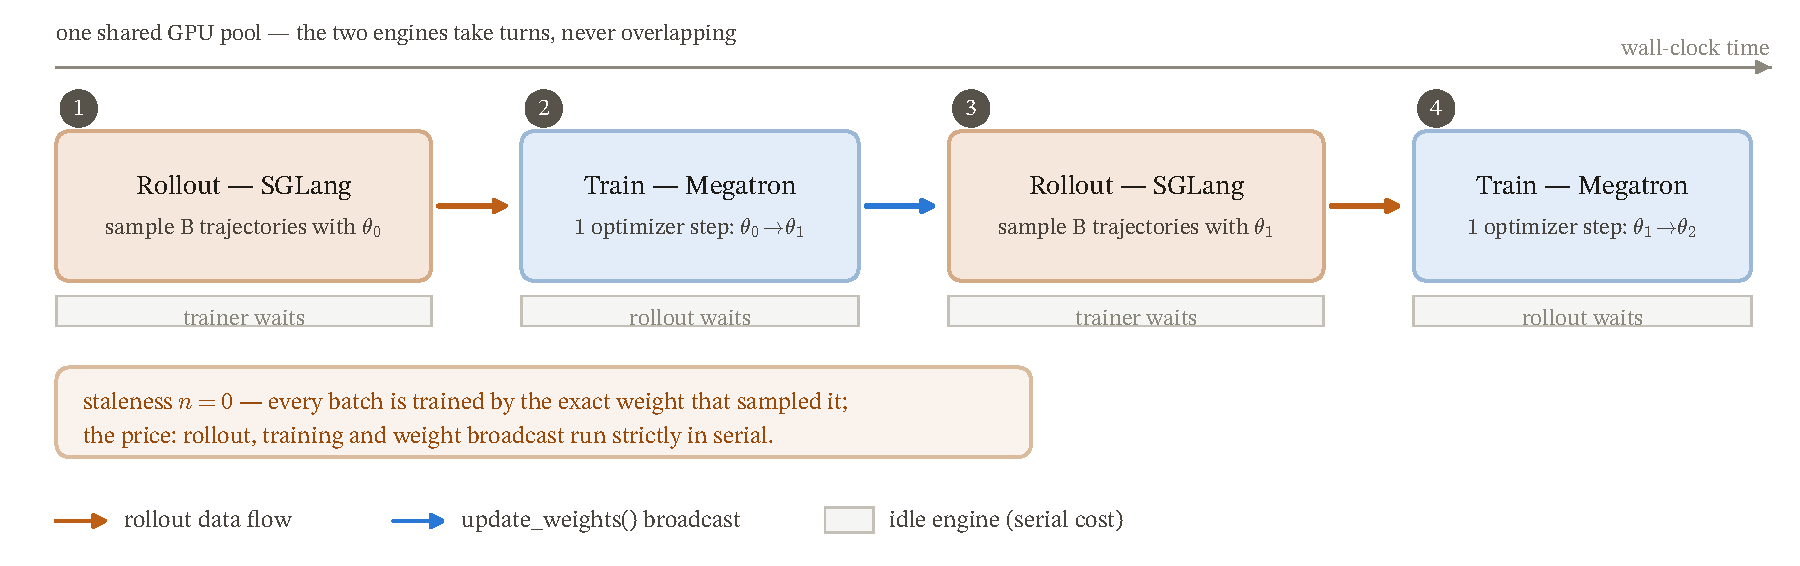
\includegraphics[width=0.88\linewidth]{figures/workflow/sync_rl_pipeline.pdf}
\caption{Synchronous RL. Rollout and training share one GPU pool and alternate in time, so each batch is consumed by the same weight version that generated it.}
\label{fig:pipeline-sync-app}
\end{figure}

\subsection{Fully asynchronous RL}
\label{app:fully-async}

Fully asynchronous RL removes the fixed batchwise handoff. Rollouts stream continuously into a queue, the trainer pulls data whenever the queue has enough completed trajectories, and new weights can be hot-swapped into the rollout engine while a response is still being decoded. A single trajectory can therefore span several policy versions before it is even enqueued, and then wait under still newer versions before it is trained. A convenient decomposition writes the realized lag as:
\begin{equation}
N_{b,t}=N_{\mathrm{PQS},b,t}+N_{\mathrm{IQS},b,t},
\label{eq:fully-async-lag}
\end{equation}
where $N_{\mathrm{PQS},b,t}$ counts the versions that elapse while the trajectory is being generated and $N_{\mathrm{IQS},b,t}$ counts the versions that elapse while the completed trajectory waits in the queue. Following \citet{dong2026staleness}, the first term grows with the response-length tail of the workload and the second depends on queue occupancy and the rollout-to-trainer throughput ratio.

This regime is important conceptually because it makes the central quantity of the paper random at the token level. Even if the system exposes one nominal queue depth or one nominal update cadence, the relevant quantity for optimization is the realized sampled mismatch $d_{b,t}=\log r_{b,t}$, not a single preconfigured scalar. This is precisely the setting in which a batch-adaptive mechanism such as \satr{} becomes more natural than a rule keyed to a fixed lag alone.

\begin{figure}[h]
\centering
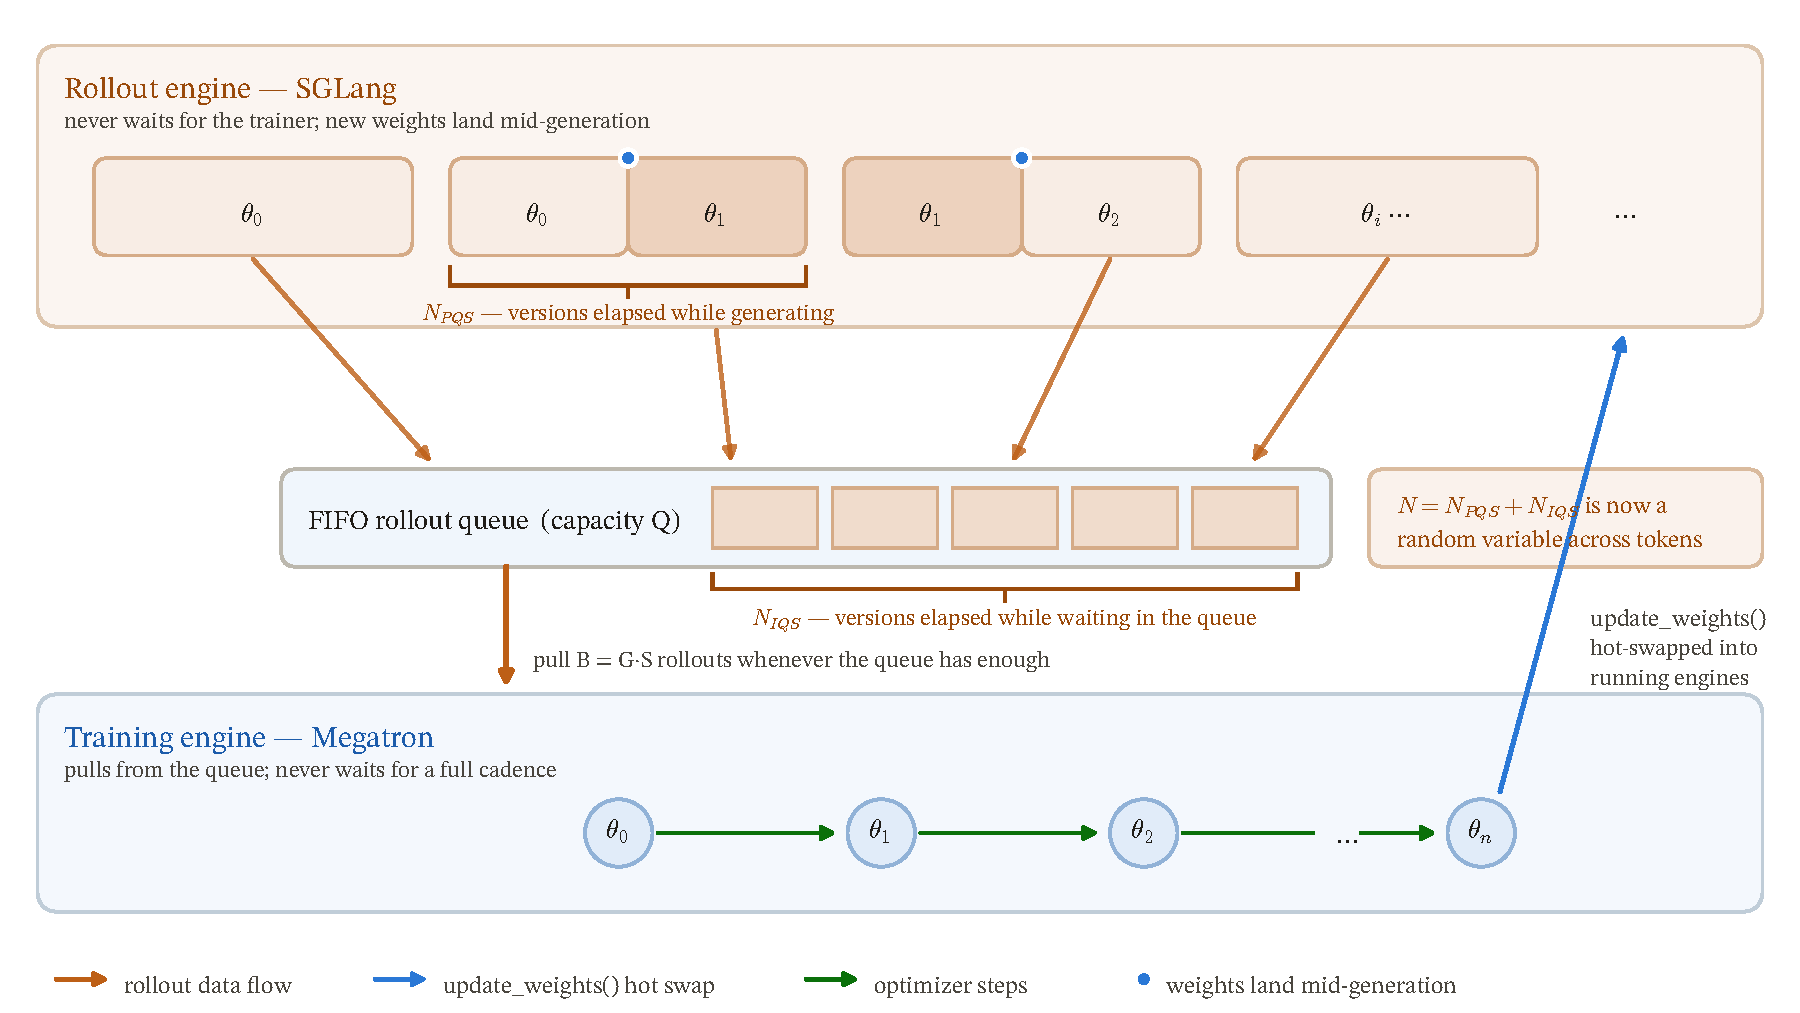
\includegraphics[width=0.88\linewidth]{figures/workflow/fully_async_rl.pdf}
\caption{Fully asynchronous RL. Rollouts stream through a queue, weights can change during generation, and the realized lag varies across tokens.}
\label{fig:pipeline-fully-app}
\end{figure}

\section{Mismatch Sources as Diagnostic Hypotheses}
\label{app:sources}

Equation~\eqref{eq:split} in the main text gives an exact two-term split of the sampled log-ratio. Write $\Delta_{b,t}^{\pi}=\log\pi^{(j)}-\log\pi^{(\ell)}$ for policy-update mismatch and $\Delta_{b,t}^{\mathrm{impl}}=\log\pi^{(\ell)}-\log\mu_{b,t}$ for implementation mismatch, both evaluated at $(y_{b,t},s_{b,t})$. Then:
\begin{equation}
d_{b,t}=\log r_{b,t}=\Delta_{b,t}^{\pi}+\Delta_{b,t}^{\mathrm{impl}}.
\label{eq:app-split}
\end{equation}
The term $\Delta_{b,t}^{\pi}$ records policy-update mismatch inside the asynchronous window. The term $\Delta_{b,t}^{\mathrm{impl}}$ records implementation mismatch between the trainer-side reference and the actual rollout engine. The purpose of the present section is not to produce a unique additive decomposition of all sources of mismatch, because such a decomposition would require additional intermediate distributions that the experiments do not log. Instead, the section records the hypotheses that are operationally useful when interpreting the measured $d_{b,t}$.

Policy updates are the most direct source. If a rollout is produced under $\theta^{(\ell)}$ and consumed after several optimizer steps, then a first-order expansion along the optimization path gives:
\begin{equation}
\log\pi^{(j)}(y_{b,t}\mid s_{b,t})-\log\pi^{(\ell)}(y_{b,t}\mid s_{b,t})
\;\approx\;\sum_{k=\ell}^{j-1}\eta\,\big\langle\nabla_\theta\log\pi(y_{b,t}\mid s_{b,t}),\,g^{(k)}\big\rangle,
\label{eq:taylor-app}
\end{equation}
with learning rate $\eta$ and update directions $g^{(k)}$. This term is exactly the object targeted by PPO-style importance reweighting. It need not be centered at zero, because consecutive updates tend to move in reward-improving directions rather than cancel each other.

Implementation mismatch remains even when the nominal weights are identical. Rollout and training may differ in fused kernels, attention kernels, KV-cache layout, numerical precision, or mixture-of-experts routing. The router case is particularly delicate because the Top-$K$ mask is a discontinuous function of the router logits. Small numerical differences can activate a different expert set and change the forward pass abruptly. Hardware differences can amplify the same effect: the same model and code path can produce train--rollout KL values that differ by orders of magnitude across GPU generations. The paper therefore treats these mechanisms as diagnostic hypotheses that explain observed mismatch and motivate stabilizers such as R3, rather than as terms of an exact decomposition used in the proof.

\section{Derivation of the Finite-Horizon Improvement Bound}
\label{app:improvement-bound}

This section collects the full derivation behind the finite-horizon trust-region discussion in Section~\ref{sec:tv}. We keep the notation of the main paper. A sequence $y=(y_1,\dots,y_T)$ is generated autoregressively from prompt $x$, the behavior policy is $\mu$, the target policy is $\pi$, rewards satisfy $|R(y)|\le\xi$, and the finite-horizon objective is $\mathcal J(\pi)=\mathbb E_{y\sim\pi}[R(y)]$. The surrogate used in the main text is:
\begin{equation}
L'_{\mu}(\pi)=\mathbb E_{y\sim\mu}\left[R(y)\sum_{t=1}^{T}\left(\frac{\pi(y_t\mid s_t)}{\mu(y_t\mid s_t)}-1\right)\right].
\label{eq:app-surrogate}
\end{equation}

\subsection{An exact performance-difference identity}
\label{app:exact-identity}

\begin{lemma}[Exact finite-horizon identity]
\label{lem:app-identity}
For any two sequence policies $\mu$ and $\pi$ with compatible support on the $\mu$-reachable states,
\begin{equation}
\mathcal J(\pi)-\mathcal J(\mu)
= L'_{\mu}(\pi)-\Delta(\mu,\pi),
\label{eq:app-identity}
\end{equation}
where
\begin{align}
L'_{\mu}(\pi)
&= \mathbb E_{y\sim\mu}\left[R(y)\sum_{t=1}^{T}\left(\frac{\pi(y_t\mid s_t)}{\mu(y_t\mid s_t)}-1\right)\right],
\label{eq:app-identity-surrogate}\\
\Delta(\mu,\pi)
&= \mathbb E_{y\sim\mu}\left[R(y)\sum_{t=1}^{T}\left(\frac{\pi(y_t\mid s_t)}{\mu(y_t\mid s_t)}-1\right)\left(1-\prod_{j=t+1}^{T}\frac{\pi(y_j\mid s_j)}{\mu(y_j\mid s_j)}\right)\right].
\label{eq:app-delta}
\end{align}
\end{lemma}

\textbf{Proof.}
Start from the definition of the return difference:
\begin{align*}
\mathcal J(\pi)-\mathcal J(\mu)
&=\mathbb E_{y\sim\pi}[R(y)]-\mathbb E_{y\sim\mu}[R(y)]\\
&=\sum_{y}\bigl(\pi(y\mid x)-\mu(y\mid x)\bigr)R(y).
\end{align*}
The sequence-probability difference admits the telescoping expansion:
\begin{equation*}
\pi(y\mid x)-\mu(y\mid x)
=\sum_{t=1}^{T}\left(\prod_{k=1}^{t-1}\mu(y_k\mid s_k)\right)
\bigl(\pi(y_t\mid s_t)-\mu(y_t\mid s_t)\bigr)
\left(\prod_{j=t+1}^{T}\pi(y_j\mid s_j)\right).
\end{equation*}
Substituting this identity and factoring out $\mu(y\mid x)$ gives:
\begin{align*}
\mathcal J(\pi)-\mathcal J(\mu)
&=\sum_{y}\mu(y\mid x)R(y)
\sum_{t=1}^{T}\left(\frac{\pi(y_t\mid s_t)}{\mu(y_t\mid s_t)}-1\right)
\left(\prod_{j=t+1}^{T}\frac{\pi(y_j\mid s_j)}{\mu(y_j\mid s_j)}\right)\\
&=\mathbb E_{y\sim\mu}\left[R(y)
\sum_{t=1}^{T}\left(\frac{\pi(y_t\mid s_t)}{\mu(y_t\mid s_t)}-1\right)
\left(\prod_{j=t+1}^{T}\frac{\pi(y_j\mid s_j)}{\mu(y_j\mid s_j)}\right)
\right].
\end{align*}
Adding and subtracting the term with the future-product replaced by $1$ yields:
\begin{align*}
\mathcal J(\pi)-\mathcal J(\mu)
&=\mathbb E_{y\sim\mu}\left[R(y)\sum_{t=1}^{T}\left(\frac{\pi(y_t\mid s_t)}{\mu(y_t\mid s_t)}-1\right)\right]\\
&\quad-\mathbb E_{y\sim\mu}\left[R(y)\sum_{t=1}^{T}\left(\frac{\pi(y_t\mid s_t)}{\mu(y_t\mid s_t)}-1\right)
\left(1-\prod_{j=t+1}^{T}\frac{\pi(y_j\mid s_j)}{\mu(y_j\mid s_j)}\right)\right],
\end{align*}
which is exactly Equations~\eqref{eq:app-identity-surrogate} and~\eqref{eq:app-delta}.
% \end{myproof}

\subsection{A sequence-level total-variation bound}
\label{app:sequence-tv}

\begin{lemma}[Sequence $D_{\mathrm{TV}}$ is bounded by cumulative one-step $D_{\mathrm{TV}}$]
\label{lem:app-sequence-tv}
Let $\mu_T(\cdot\mid s_1)$ and $\pi_T(\cdot\mid s_1)$ denote the induced sequence distributions over responses of length $T$. Then
\begin{equation}
D_{\mathrm{TV}}\bigl(\mu_T(\cdot\mid s_1)\,\|\,\pi_T(\cdot\mid s_1)\bigr)
\le
\sum_{t=1}^{T}\mathbb E_{s_t\sim\mu}\Big[D_{\mathrm{TV}}\bigl(\mu(\cdot\mid s_t)\,\|\,\pi(\cdot\mid s_t)\bigr)\Big].
\label{eq:app-sequence-tv}
\end{equation}
\end{lemma}

% \begin{myproof}
\textbf{Proof.}
Write $P(y)=\mu_T(y\mid s_1)$ and $Q(y)=\pi_T(y\mid s_1)$. Then
\begin{equation*}
2D_{\mathrm{TV}}(P\|Q)=\sum_{y}|P(y)-Q(y)|.
\end{equation*}
Using the product-difference identity:
\begin{equation*}
a_1\cdots a_T-b_1\cdots b_T
=\sum_{t=1}^{T}\left(\prod_{k=1}^{t-1}a_k\right)(a_t-b_t)\left(\prod_{j=t+1}^{T}b_j\right)
\end{equation*}
and the triangle inequality,
\begin{align*}
2D_{\mathrm{TV}}(P\|Q)
&\le \sum_{t=1}^{T}\sum_{y}
\left(\prod_{k=1}^{t-1}\mu(y_k\mid s_k)\right)
\bigl|\mu(y_t\mid s_t)-\pi(y_t\mid s_t)\bigr|
\left(\prod_{j=t+1}^{T}\pi(y_j\mid s_j)\right).
\end{align*}
For each fixed $t$, summing over $y_{t+1},\dots,y_T$ collapses the trailing product to $1$, which leaves:
\begin{align*}
2D_{\mathrm{TV}}(P\|Q)
&\le \sum_{t=1}^{T}\sum_{y_1,\dots,y_{t-1}}
\left(\prod_{k=1}^{t-1}\mu(y_k\mid s_k)\right)
\sum_{y_t}\bigl|\mu(y_t\mid s_t)-\pi(y_t\mid s_t)\bigr|.
\end{align*}
The inner sum is $2D_{\mathrm{TV}}(\mu(\cdot\mid s_t)\|\pi(\cdot\mid s_t))$, while the outer sum is the expectation over $s_t$ induced by $\mu$. Dividing by $2$ proves the claim.
% \end{myproof}

\subsection{Max-divergence and average-divergence forms}
\label{app:bound-proofs}

\begin{proposition}[Max-divergence and average-divergence bounds]
\label{prop:app-bounds}
Under the assumptions above,
\begin{equation}
\mathcal J(\pi)-\mathcal J(\mu)
\ge L'_{\mu}(\pi)-2\xi T(T-1)\bigl[D_{\mathrm{TV}}^{\max}(\mu,\pi)\bigr]^2,
\label{eq:app-max-bound}
\end{equation}
where $D_{\mathrm{TV}}^{\max}(\mu,\pi)=\sup_s D_{\mathrm{TV}}(\mu(\cdot\mid s)\|\pi(\cdot\mid s))$, and also
\begin{equation}
\mathcal J(\pi)-\mathcal J(\mu)
\ge L'_{\mu}(\pi)-4\xi\,\mathbb E_{y\sim\mu}\left[\sum_{t=1}^{T}D_{\mathrm{TV}}\bigl(\mu(\cdot\mid s_t)\,\|\,\pi(\cdot\mid s_t)\bigr)\right].
\label{eq:app-avg-bound}
\end{equation}
Equation~\eqref{eq:app-avg-bound} is the form reported in the main text as Equation~\eqref{eq:tvbound}.
\end{proposition}

\textbf{Proof of the max-divergence form}
By Lemma~\ref{lem:app-identity},
\begin{equation*}
\mathcal J(\pi)-\mathcal J(\mu)=L'_{\mu}(\pi)-\Delta(\mu,\pi).
\end{equation*}
To bound $\Delta(\mu,\pi)$, first use $|R(y)|\le\xi$:
\begin{align}
\Delta(\mu,\pi)
&\le \xi\sum_{t=1}^{T}\mathbb E_{y_{\le t}\sim\mu}\left[
\left|\frac{\pi(y_t\mid s_t)}{\mu(y_t\mid s_t)}-1\right|
\mathbb E_{y_{>t}\sim\mu(\cdot\mid s_{t+1})}
\left|1-\frac{\pi(y_{>t}\mid s_{t+1})}{\mu(y_{>t}\mid s_{t+1})}\right|
\right].
\label{eq:app-delta-step1}
\end{align}
The inner expectation is exactly twice the $D_{\mathrm{TV}}$ divergence between the future-trajectory distributions:
\begin{equation*}
\mathbb E_{y_{>t}\sim\mu(\cdot\mid s_{t+1})}
\left|1-\frac{\pi(y_{>t}\mid s_{t+1})}{\mu(y_{>t}\mid s_{t+1})}\right|
=2D_{\mathrm{TV}}\bigl(\mu_{>t}(\cdot\mid s_{t+1})\,\|\,\pi_{>t}(\cdot\mid s_{t+1})\bigr).
\end{equation*}
Applying Lemma~\ref{lem:app-sequence-tv} to this future-horizon $D_{\mathrm{TV}}$ and then upper-bounding each term by $D_{\mathrm{TV}}^{\max}(\mu,\pi)$ gives
\begin{equation*}
D_{\mathrm{TV}}\bigl(\mu_{>t}(\cdot\mid s_{t+1})\,\|\,\pi_{>t}(\cdot\mid s_{t+1})\bigr)
\le (T-t)D_{\mathrm{TV}}^{\max}(\mu,\pi).
\end{equation*}
Substituting into Equation~\eqref{eq:app-delta-step1} yields
\begin{align*}
\Delta(\mu,\pi)
&\le 2\xi D_{\mathrm{TV}}^{\max}(\mu,\pi)
\sum_{t=1}^{T}(T-t)
\mathbb E_{s_t\sim\mu}\left[\sum_{y_t}\mu(y_t\mid s_t)
\left|\frac{\pi(y_t\mid s_t)}{\mu(y_t\mid s_t)}-1\right|\right]\\
&=2\xi D_{\mathrm{TV}}^{\max}(\mu,\pi)
\sum_{t=1}^{T}(T-t)
\mathbb E_{s_t\sim\mu}\Big[2D_{\mathrm{TV}}(\mu(\cdot\mid s_t)\|\pi(\cdot\mid s_t))\Big]\\
&\le 4\xi\bigl[D_{\mathrm{TV}}^{\max}(\mu,\pi)\bigr]^2\sum_{t=1}^{T}(T-t)\\
&=2\xi T(T-1)\bigl[D_{\mathrm{TV}}^{\max}(\mu,\pi)\bigr]^2.
\end{align*}
Substituting this bound into the exact identity proves Equation~\eqref{eq:app-max-bound}.
% \end{myproof}

\textbf{Proof of the average-divergence form}
Return to Equation~\eqref{eq:app-delta-step1}. Instead of upper-bounding the future-trajectory $D_{\mathrm{TV}}$ by $(T-t)D_{\mathrm{TV}}^{\max}$, use the trivial bound $D_{\mathrm{TV}}\le 1$. This gives:
\begin{align*}
\Delta(\mu,\pi)
&\le 2\xi\sum_{t=1}^{T}\mathbb E_{y_{\le t}\sim\mu}\left[
\left|\frac{\pi(y_t\mid s_t)}{\mu(y_t\mid s_t)}-1\right|
\right]\\
&=2\xi\sum_{t=1}^{T}\mathbb E_{s_t\sim\mu}\left[
\sum_{y_t}\mu(y_t\mid s_t)
\left|\frac{\pi(y_t\mid s_t)}{\mu(y_t\mid s_t)}-1\right|
\right]\\
&=2\xi\sum_{t=1}^{T}\mathbb E_{s_t\sim\mu}\Big[2D_{\mathrm{TV}}(\mu(\cdot\mid s_t)\|\pi(\cdot\mid s_t))\Big]\\
&=4\xi\,\mathbb E_{y\sim\mu}\left[\sum_{t=1}^{T}D_{\mathrm{TV}}\bigl(\mu(\cdot\mid s_t)\,\|\,\pi(\cdot\mid s_t)\bigr)\right].
\end{align*}
Substituting this into Equation~\eqref{eq:app-identity} proves Equation~\eqref{eq:app-avg-bound}.


The two forms can be combined into the immediate corollary:
\begin{align}
\mathcal J(\pi)-\mathcal J(\mu)
\ge L'_{\mu}(\pi)-\min\Bigg(
2\xi T(T-1)\bigl[D_{\mathrm{TV}}^{\max}(\mu,\pi)\bigr]^2,
4\xi\,\mathbb E_{y\sim\mu}\left[\sum_{t=1}^{T}D_{\mathrm{TV}}\bigl(\mu(\cdot\mid s_t)\,\|\,\pi(\cdot\mid s_t)\bigr)\right]
\Bigg).
\label{eq:app-composite}
\end{align}
The max-divergence form is sharper for very small updates, whereas the average-divergence form avoids the quadratic dependence on the horizon and is more useful for long LLM responses.

\section{How Does Each Stability Approach Work in Async RL?}
\label{app:stabilizers}

The main paper introduces \satr{} as one way to adapt the sampled trust-region surrogate to the observed mismatch distribution. The larger asynchronous-RL literature can be read through the same lens. Each method chooses one mathematical object built from the observed log-ratio or from closely related quantities, such as the granularity of the ratio, the denominator, a mask, a threshold, or a clip radius, and then modifies that object. Table~\ref{tab:designspace} summarizes the design space, and the subsections below expand the methods.

\begin{table}[t]
\centering
\caption{Async-RL stabilizers in one design space. The table records which mathematical object each method modifies and whether the gate depends on the update direction $\operatorname{sign}(\hat A_t(r_t-1))$.}
\label{tab:designspace}
\small
\setlength{\tabcolsep}{5pt}
\begin{adjustbox}{max width=\textwidth}
\begin{tabular}{@{}llllll@{}}
\toprule
Method & Unit & Discriminator & Constraint & Weight $w_{b,t}$ & Direction \\
\midrule
PPO~\citep{schulman2017ppo} & token & $|r_{b,t}-1|$ & $|r_{b,t}-1|\le\varepsilon$ & $\{0,1\}$ & asymmetric \\
TRPO~\citep{schulman2015trpo} & state & $\dtv[s_t]$ & $\dtv[s_t]\le\delta_{\mathrm{TR}}$ & --- & asymmetric \\
DPPO~\citep{qi2026dppo} & token & $D_t^{\mathrm{TV}}$ & $D_t^{\mathrm{TV}}\le\delta$ & $\{0,1\}$ & asymmetric \\
DRPO~\citep{yao2026drpo} & token & $D_t^{\mathrm{TV}}$ & soft quadratic penalty & $[1-\tfrac1\delta,1+\tfrac1\delta]$ & asymmetric \\
TIS~\citep{zheng2025tis} & token & $r_{b,t}$ & one-sided cap & $\min(r_{b,t},C)$ & one-sided \\
IcePop~\citep{zhao2025icepop,hou2026sao} & token & train/inference ratio & symmetric range gate & $\{0,1\}$ or in-range weight & symmetric \\
KPop~\citep{guo2026kpop} & token & Bernoulli KL & bidirectional threshold & $\{0,1\}$ & symmetric \\
GSPO~\citep{zheng2025gspo} & sequence & $|\rho_b^{\mathrm{seq}}-1|$ & sequence clip & $\{0,1\}$ & asymmetric \\
SeqClip~\citep{tencent2025seqclip} & sequence & $\rho_b^{\mathrm{seq}}$ & $\rho_b^{\mathrm{seq}}\in[\alpha_{\mathrm{seq}},\beta_{\mathrm{seq}}]$ & $\{0,1\}$ & symmetric \\
R3~\citep{ma2025r3} & forward pass & routing mask & replay rollout Top-$K$ mask & --- & --- \\
\rowcolor{metabg!8}
\satr{} (ours) & token & $|d_{b,t}|$ and $|r_{b,t}-1|$ & adaptive clip interval & $\{0,1\}$ & asymmetric, adaptive \\
\bottomrule
\end{tabular}
\end{adjustbox}
\end{table}

\begin{figure}[p]
\centering
\begin{subfigure}[t]{0.85\textwidth}
    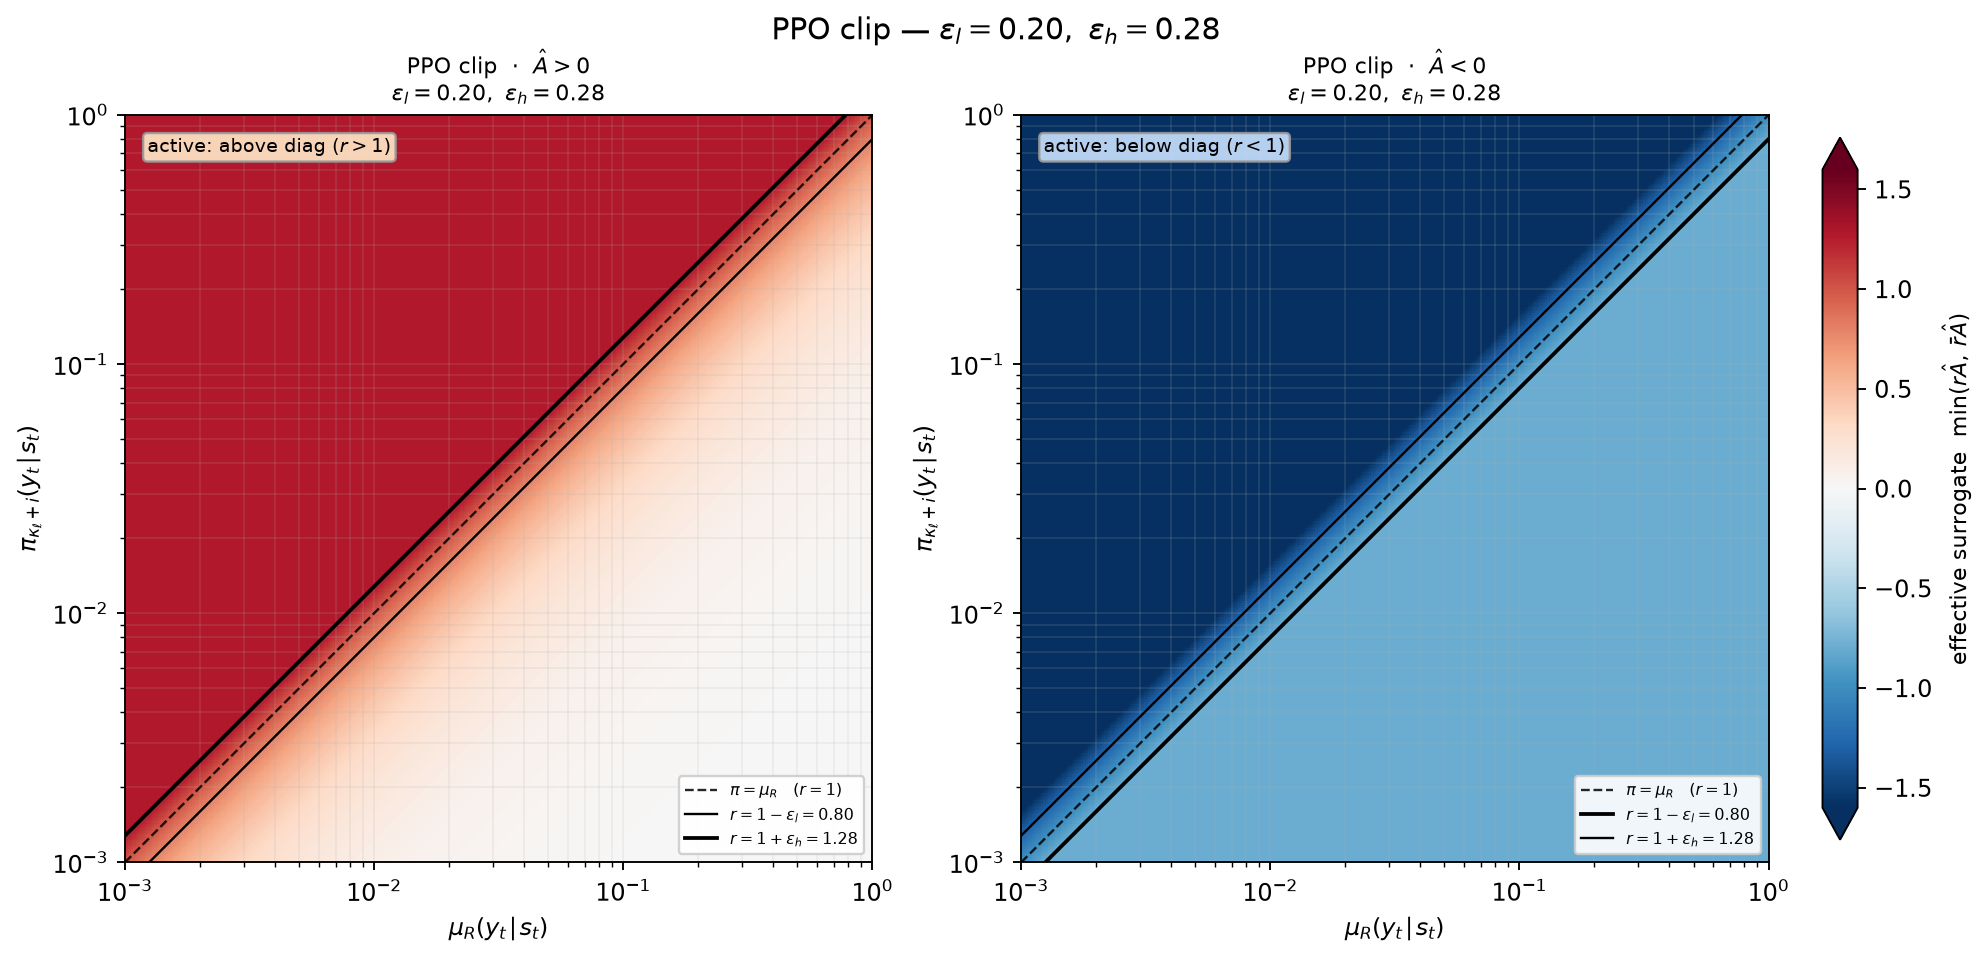
\includegraphics[width=\linewidth]{figures/asymmetric_clip_PPO.png}
    \caption{PPO}
\end{subfigure}
\caption{Asymmetric-clipping family, part I: PPO.}
\label{fig:geometry}
\end{figure}

\clearpage

\begin{figure}[p]
\centering
\begin{subfigure}[t]{0.85\textwidth}
    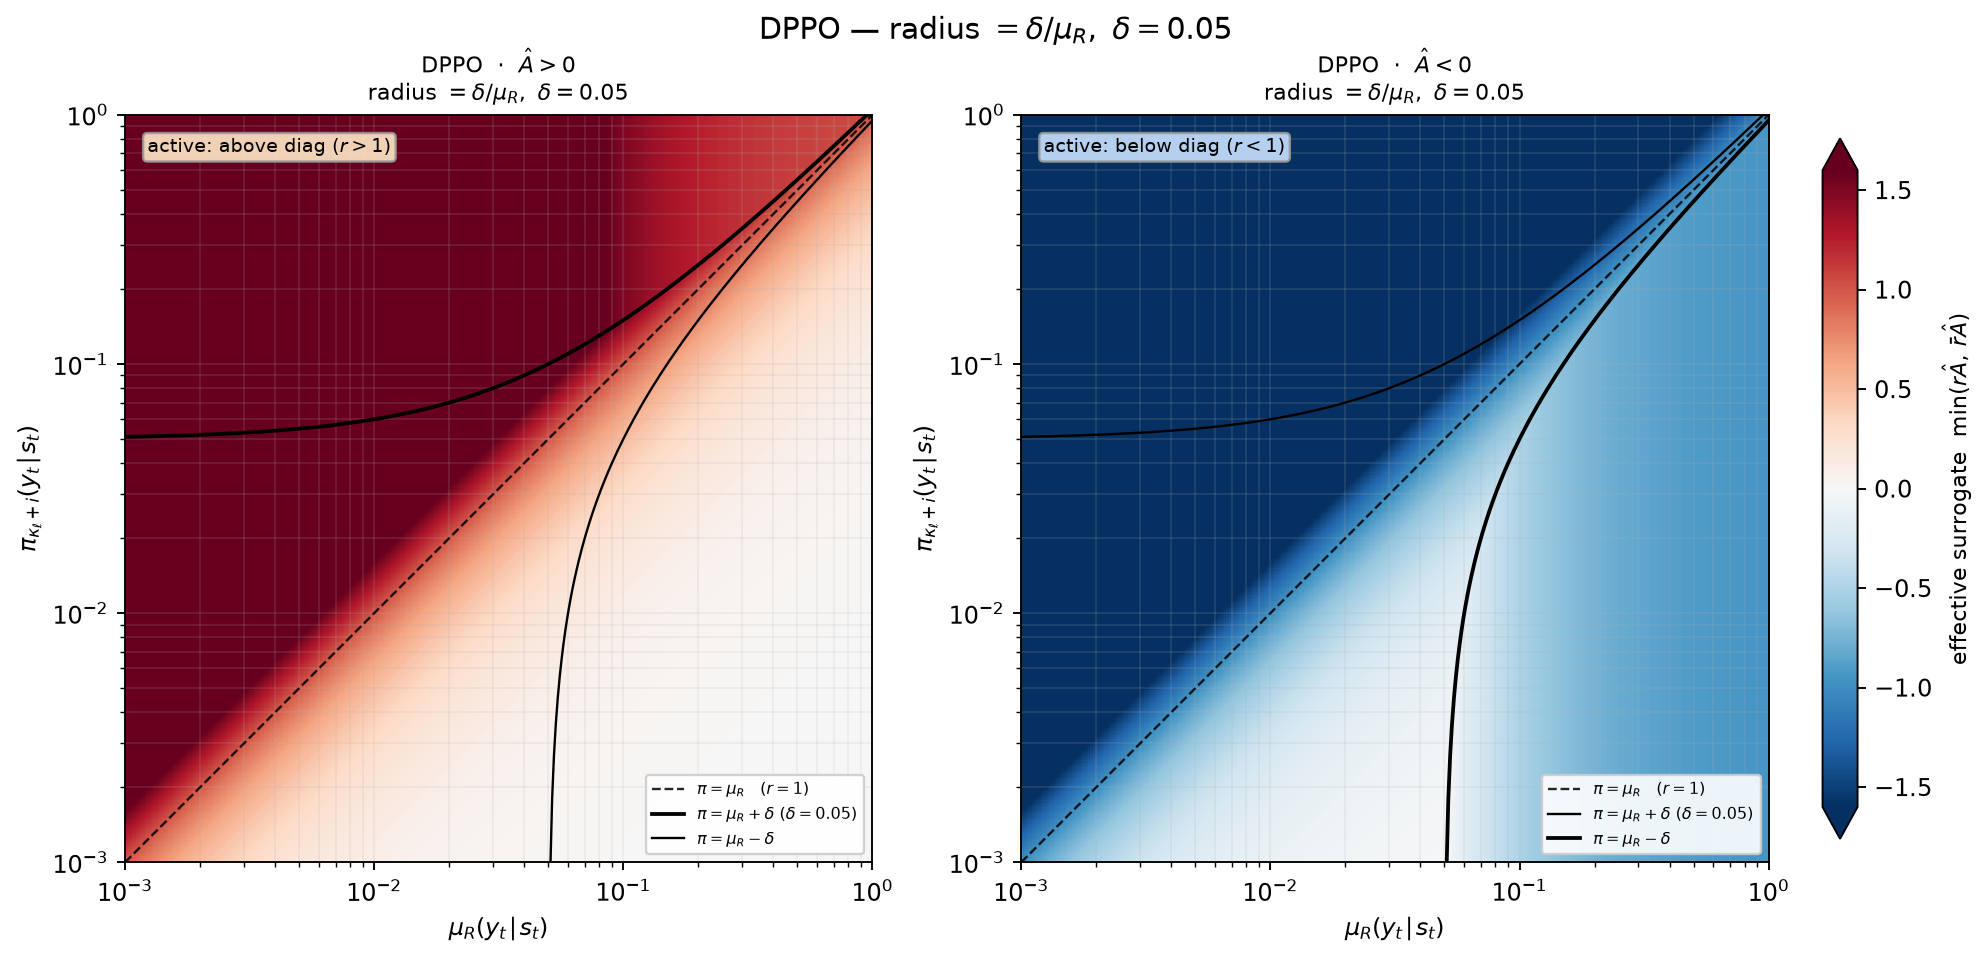
\includegraphics[width=\linewidth]{figures/asymmetric_clip_DPPO.png}
    \caption{DPPO}
\end{subfigure}\\[0.6em]
\begin{subfigure}[t]{0.85\textwidth}
    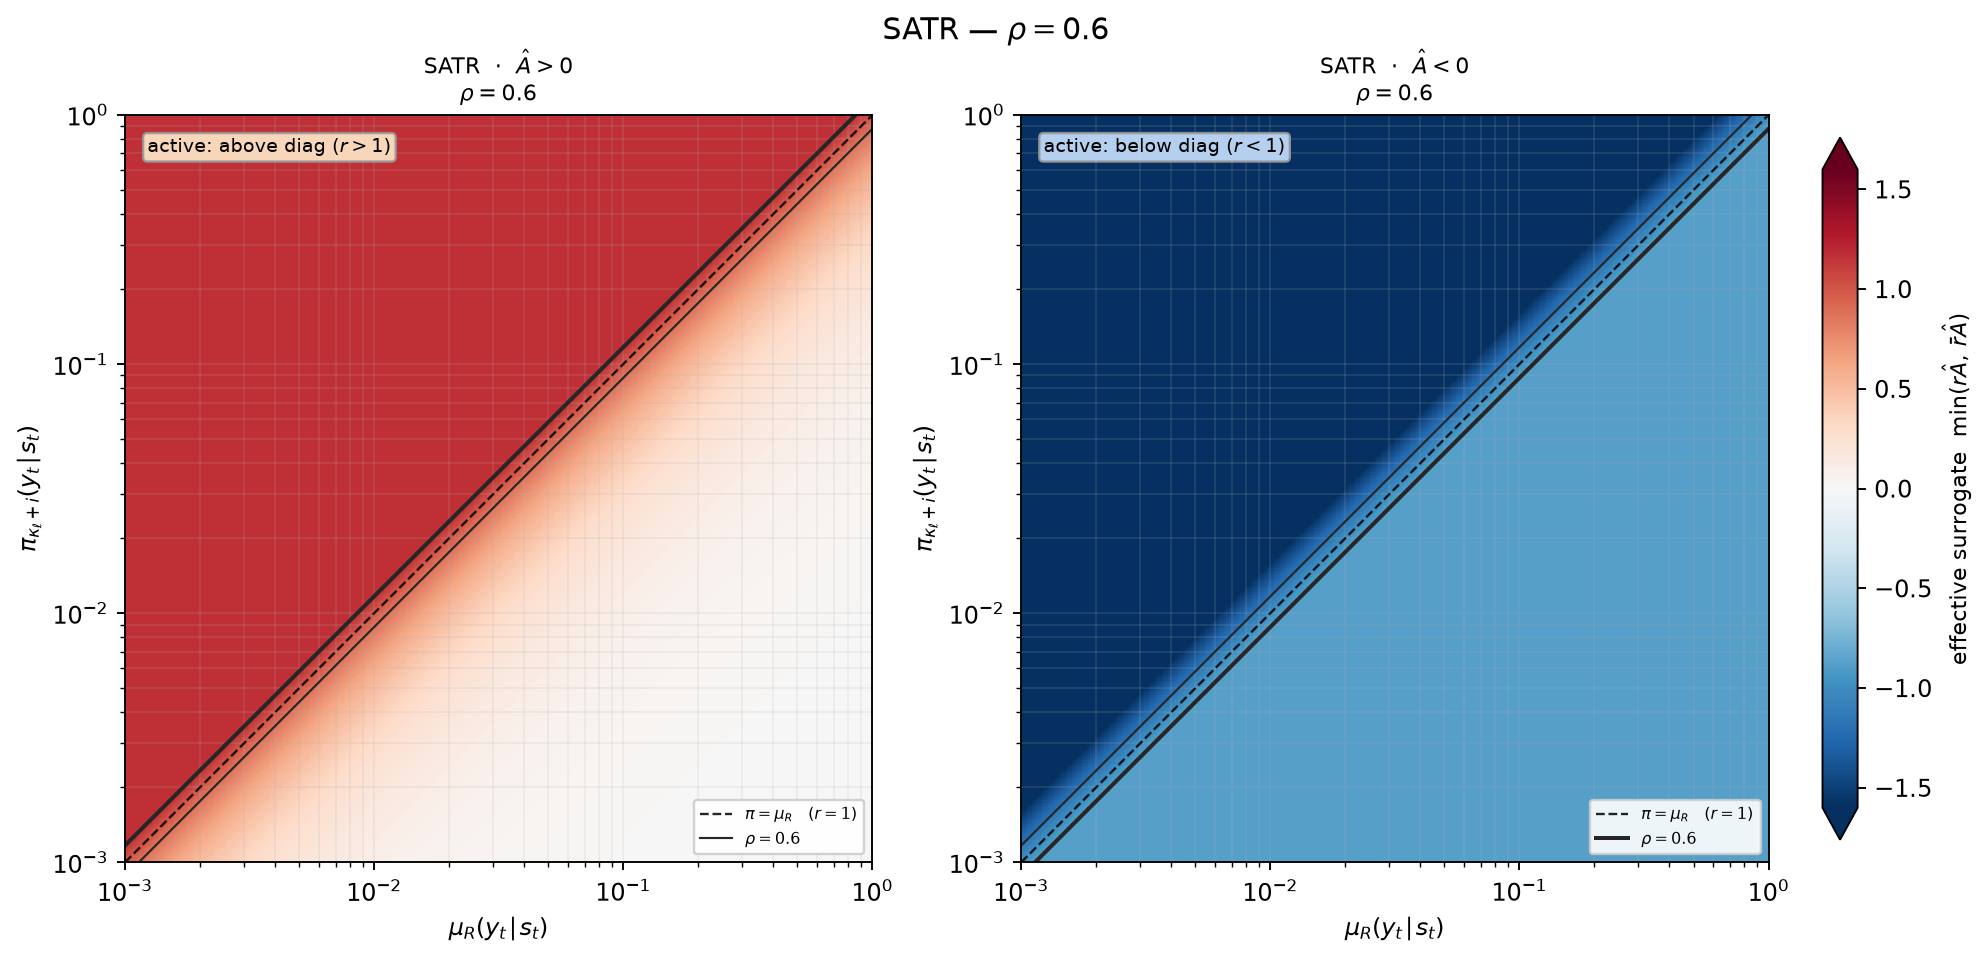
\includegraphics[width=\linewidth]{figures/asymmetric_clip_SATR.png}
    \caption{\satr{}}
\end{subfigure}
\caption{Asymmetric-clipping family, part II: DPPO and \satr{}. In this case, the contraction factor of \satr{} is set to $0.6$, which is staleness-adaptive in implementation.}
\label{fig:geometry-continued}
\end{figure}

\clearpage

\subsection{GSPO and SeqClip}
\label{app:gspo-seqclip}

GSPO moves importance weighting from the token to the response by defining the length-normalized sequence ratio:
\begin{equation}
\rho_b^{\mathrm{seq}}
=\left(\frac{\pi^{(j)}(y_b\mid x)}{\mu(y_b\mid x)}\right)^{1/T_b}
=\exp\left(\frac{1}{T_b}\sum_{t=1}^{T_b}d_{b,t}\right),
\label{eq:app-gspo}
\end{equation}
and clipping at the response level:
\begin{equation}
\mathcal S_{\mathrm{GSPO}}
=\mathbb E_{\{y_b\}\sim\mu}
\left[
\frac{1}{G}\sum_{b=1}^{G}
\min\Bigl(\rho_b^{\mathrm{seq}}\hat A_b,
\operatorname{clip}(\rho_b^{\mathrm{seq}},1-\varepsilon,1+\varepsilon)\hat A_b\Bigr)
\right].
\label{eq:app-gspo-loss}
\end{equation}
Length normalization removes the automatic exponential dependence on response length that the raw product of token ratios would induce, although token-level deviations can still reinforce or cancel. SeqClip adds a hard response-level gate:
\begin{equation}
\mathcal S_{\mathrm{SeqClip}}
=\mathbb E_{\{y_b\}\sim\mu}
\left[
\frac{1}{G}\sum_{b=1}^{G}
\mathbf 1\{\alpha_{\mathrm{seq}}\le \rho_b^{\mathrm{seq}}\le \beta_{\mathrm{seq}}\}
\min\Bigl(\rho_b^{\mathrm{seq}}\hat A_b,
\operatorname{clip}(\rho_b^{\mathrm{seq}},1-\varepsilon,1+\varepsilon)\hat A_b\Bigr)
\right].
\label{eq:app-seqclip}
\end{equation}
so responses outside a narrow interval are discarded altogether. Both methods smooth isolated token fluctuations by construction, but neither removes routing or engine mismatch, which is why the empirical combination with R3 remains relevant.

\paragraph{Empirical comparison.}
Equations~\eqref{eq:app-gspo} and~\eqref{eq:app-seqclip} define the sequence-level ratio and the hard response-level gate. Table~\ref{tab:app-exp-gspo} summarizes the matched GSPO comparison under the shared setup of Appendix~\ref{app:expdetails}. GSPO stays above GRPO at both configured lags, with $32.25$ against $31.25$ at lag $1$ and $31.46$ against $30.17$ at lag $8$. Both lag-$8$ runs later collapse in the logged window. The comparison therefore supports a difference in weighting granularity, but by itself it does not isolate which mismatch source drives the later instability. No standalone SeqClip run is reported in the current study.

\begin{table}[h]
\centering
\caption{Reported best AIME24 pass@1 for the GSPO comparison.}
\label{tab:app-exp-gspo}
\small
\begin{tabular}{@{}lcc@{}}
\toprule
Method & lag $1$ & lag $8$ \\
\midrule
GRPO & $31.25$ & $30.17^{\ddagger}$ \\
GSPO & $32.25$ & $31.46^{\ddagger}$ \\
\bottomrule
\end{tabular}
\end{table}

\subsection{Rollout Routing Replay}
\label{app:r3-detail}

R3 addresses mismatch from discrete MoE routing. Even at nominally identical weights, SGLang and Megatron can choose different Top-$K$ experts for the same token, and asynchronous updates add another source of variation. R3 replays the rollout-time Top-$K$ mask while keeping the current trainer logits in the softmax denominator,
\begin{equation}
g^{(j)}_{\mathrm{replay},e}
=\frac{I^{(\ell)}_{\mathrm{infer},e}\,\exp\bigl(z^{(j)}_{\mathrm{train},e}\bigr)}
{\sum_{e'}I^{(\ell)}_{\mathrm{infer},e'}\,\exp\bigl(z^{(j)}_{\mathrm{train},e'}\bigr)},
\qquad
\mathbf h^{(j)}_{\mathrm{replay}}
=\sum_{e=1}^{M}g^{(j)}_{\mathrm{replay},e}\,\mathcal E_e^{(j)}(\mathbf h_{\mathrm{train}}).
\label{eq:r3}
\end{equation}
This aligns the discrete expert set with rollout while still allowing gradients to flow through the current router. It does not reproduce the entire rollout forward pass, since hidden states, logits, expert weights, and downstream layers may still differ, but it removes one important mismatch source at the routing branch.

\paragraph{Empirical comparison.}
Equation~\eqref{eq:r3} defines the replayed routing gate. Table~\ref{tab:app-exp-r3} summarizes the matched R3 comparison. The strongest gain appears for the GSPO pairing, which reaches $34.00$ at lag $1$ and $33.13$ at lag $8$. In the reported summary, the lag-$8$ GSPO w/ R3 run is not marked as a later-collapse setting. GRPO w/ R3 improves over GRPO at lag $1$, but remains below GSPO w/ R3 at both lags. These numbers are consistent with routing replay reducing MoE routing mismatch on the reported stack, but they do not establish a unique causal path.

\begin{table}[h]
\centering
\caption{Reported best AIME24 pass@1 for the R3 comparison.}
\label{tab:app-exp-r3}
\small
\begin{tabular}{@{}lcc@{}}
\toprule
Method & lag $1$ & lag $8$ \\
\midrule
GRPO & $31.25$ & $30.17^{\ddagger}$ \\
GSPO & $32.25$ & $31.46^{\ddagger}$ \\
GRPO w/ R3 & $31.83$ & $29.58$ \\
GSPO w/ R3 & $34.00$ & $33.13$ \\
\bottomrule
\end{tabular}
\end{table}

\subsection{TIS, IcePop, and KPop}
\label{app:token-stabilizers}

TIS, IcePop, and KPop act on sampled tokens rather than whole responses. TIS is the mildest intervention: it caps only the overshoot side of the importance weight:
\begin{equation}
w_{b,t}^{\mathrm{TIS}}=\min\bigl(r_{b,t},C\bigr),
\qquad
\mathcal S_{\mathrm{TIS}}
=\mathbb E\left[\sum_{b,t}\operatorname{sg}[w_{b,t}^{\mathrm{TIS}}]\hat A_{b,t}\log\pi^{(j)}(y_{b,t}\mid s_{b,t})\right].
\label{eq:app-tis}
\end{equation}
It changes gradient magnitude but does not alter the clip interval. IcePop instead applies a two-sided gate to the train-engine versus inference-engine ratio:
\begin{equation}
k_{b,t}=\frac{\tilde\mu_{b,t}(y_{b,t}\mid s_{b,t})}{\mu_{b,t}(y_{b,t}\mid s_{b,t})},
\qquad
M_{b,t}^{\mathrm{IcePop}}=k_{b,t}\,\mathbf 1\{\alpha\le k_{b,t}\le\beta\},
\label{eq:app-icepop}
\end{equation}
which is often simplified to a binary in-range mask. KPop replaces raw ratios with a Bernoulli-KL test:
\begin{equation}
D_{\mathrm{KL}}^{\mathrm{Bern}}(p\|q)=p\log\frac{p}{q}+(1-p)\log\frac{1-p}{1-q},
\qquad
M_{b,t}^{\mathrm{KPop}}
=\mathbf 1\bigl\{D_{\mathrm{KL}}^{\mathrm{Bern}}(p_{b,t}^{\pi}\|p_{b,t}^{\mu})\le\phi\bigr\}
\mathbf 1\bigl\{D_{\mathrm{KL}}^{\mathrm{Bern}}(p_{b,t}^{\mu}\|p_{b,t}^{\pi})\le\phi\bigr\}.
\label{eq:app-kpop}
\end{equation}
where $p_{b,t}^{\pi}$ and $p_{b,t}^{\mu}$ are the trainer- and rollout-side probabilities of the sampled token. IcePop and KPop are symmetric in direction: they may discard tokens whose local gradient would move the sampled ratio back toward the behavior reference.

\paragraph{Empirical comparison.}
Equations~\eqref{eq:app-tis}--\eqref{eq:app-kpop} summarize the token-level mechanisms. The current study reports matched runs for TIS and its compositions with R3, but not standalone AIME24 grids for IcePop or KPop. Table~\ref{tab:app-exp-tis} shows that the TIS family remains in a relatively narrow band from $31.21$ to $32.92$ across the two configured lags, and none of these runs is marked as a later-collapse setting. The strongest lag-$8$ value in this family is $32.92$ for GSPO w/ TIS w/ R3.

\begin{table}[h]
\centering
\caption{Reported best AIME24 pass@1 for the TIS comparison.}
\label{tab:app-exp-tis}
\small
\begin{tabular}{@{}lcc@{}}
\toprule
Method & lag $1$ & lag $8$ \\
\midrule
GRPO w/ TIS & $31.62$ & $31.46$ \\
GSPO w/ TIS & $32.88$ & $31.21$ \\
GRPO w/ TIS w/ R3 & $31.79$ & $31.79$ \\
GSPO w/ TIS w/ R3 & $31.88$ & $32.92$ \\
\bottomrule
\end{tabular}
\end{table}

\subsection{Asymmetric clipping}
\label{app:asymclip}

The comparison most relevant for this paper is between PPO, DPPO, and \satr{}, since all three act directly on sampled-token updates through an asymmetric trust-region-style gate. For a fixed sampled token with ratio $r_t$ and advantage $\hat A_t$, the unclipped surrogate has derivative $\hat A_t$ with respect to $r_t$, so the sign of $\hat A_t$ determines the locally preferred direction. Relative to $r_t=1$, the sampled update is locally diverging when $\operatorname{sign}(\hat A_t(r_t-1))>0$ and locally converging when $\operatorname{sign}(\hat A_t(r_t-1))<0$. The three methods differ in how they decide when an outward move should be stopped: PPO uses a fixed ratio interval, DPPO replaces that fixed interval by a token-dependent threshold induced by a sampled $D_{\mathrm{TV}}$ bound, and \satr{} further makes the effective clip radius contract on the high-staleness tail while leaving pull-back updates open.

Away from the kinks, PPO therefore keeps the gate:
\begin{equation}
M_t^{\mathrm{PPO}}=\mathbf 1\Bigl\{\operatorname{sign}(\hat A_t(r_t-1))\le 0\ \vee\ |r_t-1|\le\varepsilon\Bigr\},
\label{eq:app-ppo-mask}
\end{equation}
which clips only outward moves beyond the nominal interval and always preserves pull-back updates.

DPPO keeps the same directional logic but changes the discriminator. Under the sampled $D_{\mathrm{TV}}$ discriminator:
\begin{equation}
D_t^{\mathrm{TV}}=\bigl|\pi^{(j)}(y_t\mid s_t)-\mu(y_t\mid s_t)\bigr|=\mu(y_t\mid s_t)\,|r_t-1|,
\label{eq:app-bintv}
\end{equation}
so $D_t^{\mathrm{TV}}\le\delta$ is equivalent to:
\begin{equation}
|r_t-1|\le \frac{\delta}{\mu(y_t\mid s_t)}.
\label{eq:app-dppo-eps}
\end{equation}
The induced mask is:
\begin{equation}
M_t^{\mathrm{DPPO}}
=\mathbf 1\Bigl\{\operatorname{sign}(\hat A_t(r_t-1))\le 0\ \vee\ |r_t-1|\le\delta/\mu(y_t\mid s_t)\Bigr\},
\label{eq:app-dppo-mask}
\end{equation}
which is loose on long-tail tokens and tight on head tokens. SPO and DRPO replace hard clipping with quadratic penalties. SPO uses:
\begin{equation}
\mathcal S_{\mathrm{SPO}}(\pi)
=\mathbb E\left[\sum_t\left(r_t\hat A_t-\frac{|\hat A_t|}{2\varepsilon}(r_t-1)^2\right)\right],
\label{eq:app-spo}
\end{equation}
whose stationary point lies at $r_t^{\star}=1+\operatorname{sign}(\hat A_t)\varepsilon$, exactly on PPO's boundary. DRPO makes the same replacement in DPPO's sampled $D_{\mathrm{TV}}$ geometry:
\begin{equation}
\mathcal S_{\mathrm{DRPO}}(\pi^{(j)})
=\mathbb E_{y\sim\mu}\left[\sum_t\left(r_t\hat A_t-\frac{|\hat A_t|}{2\delta}\,\mu(y_t\mid s_t)(r_t-1)^2\right)\right].
\label{eq:app-drpo}
\end{equation}
Unlike \satr{}, however, their thresholds are fixed in advance rather than inferred from the current mismatch tail.

\paragraph{Empirical comparison.}
Equations~\eqref{eq:app-dppo-mask} and~\eqref{eq:app-drpo} place DPPO and DRPO inside the asymmetric-clipping family. Table~\ref{tab:app-exp-dppo} summarizes the reported DPPO comparison. DPPO reaches $33.96$ at lag $1$ and $32.71$ at lag $8$. It stays above the GRPO baseline at both lags and outside the runs marked as later collapse. This is consistent with a sampled $D_{\mathrm{TV}}$ gate improving stability on the reported stack, but it does not explain the remaining gap to \satr-GSPO w/ R3 or even to \satr-GRPO w/ R3.

\begin{table}[h]
\centering
\caption{Reported best AIME24 pass@1 for the DPPO comparison.}
\label{tab:app-exp-dppo}
\small
\begin{tabular}{@{}lcc@{}}
\toprule
Method & lag $1$ & lag $8$ \\
\midrule
GRPO & $31.25$ & $30.17^{\ddagger}$ \\
GSPO & $32.25$ & $31.46^{\ddagger}$ \\
DPPO & $33.96$ & $32.71$ \\
\bottomrule
\end{tabular}
\end{table}

\subsection{Top-$p$ configuration}
\label{app:topp}

Support mismatch appears when rollout truncates the behavior distribution but training evaluates an untruncated target policy. If rollout uses top-$p$ below $1$, actions outside the nucleus have zero behavior probability, so absolute continuity $\pi^{(j)}\ll\mu_{b,t}$ can fail. One fix is to replay the rollout truncation mask inside the trainer softmax, as in MAI-Thinking-1~\citep{microsoft2025mai}. If $\mathcal T_{b,t}\subseteq\mathcal V$ denotes the rollout nucleus, training uses:
\begin{equation}
\tilde{\mathrm{logit}}_{b,t}(a)=
\begin{cases}
\mathrm{logit}_{b,t}(a), & a\in\mathcal T_{b,t},\\
-\infty, & a\notin\mathcal T_{b,t},
\end{cases}
\qquad
\pi^{(j)}(a\mid s_{b,t})=\operatorname{softmax}(\tilde{\mathrm{logit}}_{b,t})(a).
\label{eq:app-top-p-replay}
\end{equation}
Our experiments use the simpler alternative of disabling truncation at rollout entirely by setting temperature $1.0$, top-$p$ to $1.0$, and top-$k$ to $-1$, so the rollout support matches the full vocabulary.

\paragraph{Empirical note.}
Equation~\eqref{eq:app-top-p-replay} gives the replayed support mask when rollout truncation is enabled. The companion analysis does not report a separate AIME24 grid for top-$p$. In the present experiments we instead disable truncation at rollout with temperature $1.0$, top-$p$ set to $1.0$, and top-$k$ set to $-1$, so rollout support matches the full vocabulary. Under this configuration, the reported trainer-to-rollout KL remains on the order of $10^{-3}$, which is comparable to the post-R3 regime on the same stack.

\subsection{Using rollout log probabilities}
\label{app:rollout-lp}

A separate choice concerns the denominator of the sampled ratio. Standard asynchronous PPO/GRPO often uses the trainer-side recomputation $\tilde\mu_{b,t}$ as the reference log-probability. Replacing it with the rollout log-probability restores the actual behavior denominator:
\begin{equation}
\log\tilde\mu_{b,t}(y_{b,t}\mid s_{b,t})\leftarrow \log\mu_{b,t}(y_{b,t}\mid s_{b,t}),
\qquad
r_{b,t}^{\mathrm{rollout-lp}}
=\exp\Bigl(\log\pi^{(j)}(y_{b,t}\mid s_{b,t})-\log\mu_{b,t}(y_{b,t}\mid s_{b,t})\Bigr)=r_{b,t}.
\label{eq:app-rollout-lp}
\end{equation}
Under the support condition, this is the denominator required by the importance-sampling identity. It may also increase the observed variance of sampled ratios, because implementation mismatch is no longer absorbed by trainer-side recomputation. The change therefore exposes mismatch more faithfully, but does not reduce policy-version lag by itself.

\paragraph{Empirical comparison.}
Equation~\eqref{eq:app-rollout-lp} defines the denominator switch. Table~\ref{tab:app-exp-rolloutlp} records the observed variance of the sampled log-ratio with and without rollout log probabilities. The switch exposes more implementation mismatch to the optimizer and increases the measured variance in the reported runs. This is a property of the estimator used in optimization rather than a change to the deterministic population bound itself.

\begin{table}[h]
\centering
\caption{Observed variance of the sampled log-ratio when rollout log probabilities are used as the denominator.}
\label{tab:app-exp-rolloutlp}
\small
\begin{tabular}{@{}lcc@{}}
\toprule
Method & lag $1$ & lag $8$ \\
\midrule
GRPO & $2.6\times 10^{-4}$ & $1.4\times 10^{-4}$ \\
GRPO w/ rollout log probabilities & $3.2\times 10^{-4}$ & $2.7\times 10^{-4}$ \\
\bottomrule
\end{tabular}
\end{table}

\section{Experimental Details}
\label{app:expdetails}

The backbone is Qwen3-30B-A3B-Base, an MoE model with $48$ layers, hidden size $2048$, $128$ experts with Top-$8$ routing, MoE-FFN width $768$, a softmax router, no auxiliary routing loss, and RoPE base $10^6$. The benchmark is AIME24 with $30$ problems. Each evaluation uses $16$ samples per problem, a $30$k response cap, top-$p$ set to $1$, and is run every five training iterations. Each logged evaluation score averages four evaluation runs, and the base-model reference is $9.38$.

All experiments run on the slime asynchronous RL framework with SGLang as the rollout engine and Megatron as the trainer. The configured lag is controlled at $n\in\{1,8\}$, with a weight-broadcast interval of $8$ for the lag-$8$ runs. All runs in a comparison share the optimizer, data, and reward. Table~\ref{tab:main-combined} reports both the best logged AIME24 checkpoint over the training window and the corresponding last-epoch sampled mismatch values. The symbol $\ddagger$ marks runs that later collapse and do not recover in the logged window, even though the best-so-far checkpoint is still reported.

Training data consists of the union of DAPO-Math-17k~\citep{yu2025dapoopensourcellmreinforcement} and Dolci-RL-Zero-Math-7B~\citep{olmo2026olmo3}, with $30{,}712$ prompts in total. We use a chat template, rollout shuffling, and balanced sampling. The reward is the rule-based PrimeMath verifier with multi-pattern answer extraction, Hendrycks-MATH normalization, and SymPy equivalence checking. Optimization uses Adam with $\beta_1=0.9$, $\beta_2=0.98$, and constant learning rate $10^{-6}$, without warmup or decay. Each iteration consumes $256$ prompts and $16$ samples per prompt, for $4096$ responses in total, with one minor step per broadcast and $544$ rollout iterations. Rollout and evaluation use a maximum response length of $32$k tokens and dynamic batching with a $32$k per-GPU token cap. Sampling is performed at temperature $1.0$, top-$p$ set to $1.0$, and top-$k$ set to $-1$, so the rollout distribution has full-vocabulary support. The base clip radii are $(\elow,\ehigh)=(0.2,0.2)$. The KL regularizer is low-variance KL with coefficient $10^{-3}$, and the entropy bonus is zero. For \satr{}, we use the Hill kernel with exponent $2$ and reference quantile $0.90$. Hardware consists of one node with eight GPUs, using GPU0--3 for training and GPU4--7 for rollout, with TP$=4$, PP$=1$, CP$=1$, EP$=4$, ETP$=1$, sequence parallelism, bf16 arithmetic with fp32 gradient all-reduce and fp32 attention softmax, the FlashAttention backend, and SGLang memory fraction set to $0.85$.

The per-method settings differ only in the ratio and KL granularity and in the clipping or gating rule. GRPO uses per-token ratios and per-token KL with the standard asymmetric PPO clip. GSPO keeps the same outer objective but replaces the token ratio and KL by a sequence-level ratio and a sequence-level mean KL that is all-gathered and broadcast to all active tokens of the response. DPPO multiplies the GRPO clip by a hard mask that zeros sampled tokens only when the local update is outward and the sampled $D_{\mathrm{TV}}$ discriminator exceeds its threshold; in the reported runs, this is the DPPO-$D_{\mathrm{TV}}$ variant and the threshold is $10^{-3}$. When \satr{} is layered on top of any base recipe, it contracts the shared radii using the ratio scalar of that recipe, namely the token ratio for GRPO and the broadcast sequence ratio for GSPO, and it is bit-identical to the base loss when disabled. R3 and TIS are toggled independently and therefore compose with both fixed-clip and adaptive-clip objectives.

\paragraph{Metrics and statistical scope}
\label{app:metrics-scope}
We report (i) the best-observed AIME24 pass@1 over the logged training window; AIME24 has $30$ problems, each evaluation uses $16$ samples per problem, runs every five training iterations, and each logged score averages four evaluation runs (base-model reference: $9.38$); and (ii) the sampled training--inference mismatch:
\begin{equation}
\dpi\;=\;\E_{(b,t)\in\mathcal T_{\mathrm{act}}}\big|\log r^{\mathrm{tok}}_{b,t}\big|,
\label{eq:mismatch-metric}
\end{equation}
computed from the token ratio of Equation~\eqref{eq:gspo-ratio} for all methods including GSPO, reported in the lower panel of Table~\ref{tab:main-combined} and as paired per-step curves in Figure~\ref{fig:drift-pair}. Every configuration is a single training seed, so each cell is one run: the numbers are a snapshot rather than confidence-interval estimates, and where the text calls two $\dpi$ values ``close'' we mean within the trailing-25\% within-run fluctuation, not a multi-seed test. Lower $\dpi$ means less observed sampled mismatch; it is not a full-$D_{\mathrm{TV}}$ measurement and not by itself a return ranking.

\begin{table}[h]
\centering
\caption{Per-method reproducible hyper-parameters. All other settings are shared and summarized above.}
\label{tab:hparams}
\small
\setlength{\tabcolsep}{7pt}
\begin{tabular}{@{}lccc@{}}
\toprule
Hyper-parameter & GRPO & GSPO & DPPO \\
\midrule
advantage estimator & GRPO & GSPO & DPPO \\
ratio / KL granularity & per-token & per-sequence & per-token \\
$(\elow,\ehigh)$ & $(0.2,0.2)$ & $(0.2,0.2)$ & $(0.2,0.2)$ \\
KL-loss coefficient & $10^{-3}$ & $10^{-3}$ & $10^{-3}$ \\
KL-loss type & low-variance KL & low-variance KL & low-variance KL \\
entropy coefficient & $0$ & $0$ & $0$ \\
extra mechanism & $-$ & sequence-level KL all-gather & $D_{\mathrm{TV}}$ hard mask $\delta=10^{-3}$ \\
needs rollout log-prob & no & no & yes \\
\bottomrule
\end{tabular}
\end{table}

Each cell of Table~\ref{tab:main-combined} is a single run at a fixed seed, so the empirical scope is intentionally narrow. The $\dpi$ curves in Figure~\ref{fig:drift-pair} are raw per-step logs at a four-step stride without smoothing. Steady-state values quoted in the caption average the trailing $25\%$ of each run, whereas the lower $\dpi$ block of Table~\ref{tab:main-combined} reports last-epoch means, so the two summaries can differ slightly for the same configuration. At lag $1$, the trailing-$25\%$ values are approximately $0.0102$ for GRPO, $0.0103$ for DPPO, $0.0101$ for GSPO w/ TIS, $0.0104$ for \satr-GSPO, $0.0061$ for GSPO w/ TIS w/ R3, $0.0055$ for GRPO w/ R3, $0.0057$ for GSPO w/ R3, and $0.0058$ for \satr-GSPO w/ R3. At lag $8$, the corresponding values are approximately $0.0068$ for GSPO w/ TIS w/ R3, $0.0073$ for GSPO w/ R3, $0.0085$ for \satr-GRPO w/ R3, $0.0097$ for GRPO w/ R3, and $0.0108$ for \satr-GSPO, while the remaining shown runs lie roughly in the $0.0103$--$0.0131$ range and the GSPO baseline diverges beyond the plotted axis.

\FloatBarrier

\section{\satr{} Runtime Diagnostics}
\label{app:monitor}

\begin{table}[h]
\centering
\caption{Diagnostics emitted at every optimizer step by the adaptive rule in Equations~\eqref{eq:gate}--\eqref{eq:adaptive-eps}. They describe the implemented gate on sampled tokens rather than full-vocabulary $D_{\mathrm{TV}}$.}
\label{tab:monitor}
\small
\begin{tabular}{@{}ll@{}}
\toprule
Quantity & Meaning \\
\midrule
$\E_{(b,t)\in\mathcal T_{\mathrm{act}}}[\elow\,c_{-,b,t}]$ & Mean effective lower radius on active sampled tokens. \\
$\E_{(b,t)\in\mathcal T_{\mathrm{act}}}[\ehigh\,c_{+,b,t}]$ & Mean effective upper radius on active sampled tokens. \\
$\E_{(b,t)\in\mathcal T_{\mathrm{act}}}\big[\mathbf 1\{q>0,\ |d_{b,t}|>q\}\big]$ & Realized gate rate; ties can make it smaller than $10\%$. \\
$\min_{(b,t)\in\mathcal T_{\mathrm{act}}}c_{\pm,b,t}$ & Strongest contraction applied to a sampled token in the microbatch. \\
$q$ & Detached microbatch quantile reference from Equation~\eqref{eq:quantile}. \\
\bottomrule
\end{tabular}
\end{table}
